\documentclass[12pt]{article}
\usepackage{enumitem}
%\usepackage[T1]{fontenc}
\usepackage[auth-sc,affil-sl]{authblk}
\usepackage{amsmath}
\usepackage{graphicx}
\usepackage{color}
\usepackage[toc,page]{appendix}
%\usepackage{enumerate}
\usepackage[round]{natbib}
%\usepackage{url} % not crucial - just used below for the URL 
%\usepackage{amsthm}
\usepackage{amssymb}
\usepackage{graphicx}
\usepackage{epstopdf}
\usepackage{hyperref}
\usepackage{alltt}
\usepackage{listings}
\usepackage{array}
\usepackage[noline, boxed, linesnumbered, procnumbered, titlenumbered]{algorithm2e}
%\usepackage[firstpage]{draftwatermark}
\usepackage[margin=1in]{geometry}  %%jcgs has own margins
\usepackage{lmodern}
\usepackage{caption}
\usepackage{subcaption}

%\pdfminorversion=4
% NOTE: To produce blinded version, replace "0" with "1" below.
\newcommand{\blind}{0}

\newcommand{\secref}[1]{Section~\ref{#1}}
\newcommand{\appdxref}[1]{Appendix~\ref{#1}}
\newcommand{\tblref}[1]{Table~\ref{#1}}
\newcommand{\figref}[1]{Figure~\ref{#1}}
\newcommand{\thmref}[1]{Theorem~\ref{#1}}
\newcommand{\algref}[1]{Algorithm~\ref{#1}}
\newcommand{\funref}[1]{Function~\ref{#1}}
\newcommand{\eqnref}[1]{Equation~\ref{#1}}
\newcommand{\listingref}[1]{Listing~\ref{#1}}

\newcommand{\eg}{{\em e.g.}}
\newcommand{\ith}{$i^{th}$}
\newcommand{\cut}[1]{}
\newcommand{\todo}[1]{{{\color{red}{[#1]}}}}

\newcommand{\Ex}{\mathop{\mathbb{E}}}
\newcommand{\Imp}{\mathbf{I}}

\newcommand{\spd}{\fontfamily{cmr}\textsc{\small StratPD}}
\newcommand{\cspd}{\fontfamily{cmr}\textsc{\small CatStratPD}}
\newcommand{\xnc}{$x_{\overline{c}}$}
\renewcommand{\xi}{x^{(i)}}
\newcommand{\xnC}{$x_{\overline{C}}$}

\setlist[enumerate]{itemsep=-1mm}

% DON'T change margins - should be 1 inch all around.
\cut{
\addtolength{\oddsidemargin}{-.5in}%
\addtolength{\evensidemargin}{-.5in}%
\addtolength{\textwidth}{1in}%
\addtolength{\textheight}{1.3in}%
\addtolength{\topmargin}{-.8in}%
}

\begin{document}

\def\spacingset#1{\renewcommand{\baselinestretch}%
{#1}\small\normalsize} \spacingset{1}


%%%%%%%%%%%%%%%%%%%%%%%%%%%%%%%%%%%%%%%%%%%%%%%%%%%%%%%%%%%%%%%%%%%%%%%%%%%%%%

\if0\blind
{
  \title{\bf Tech Report: Model-Free Feature Importance}

  \author{Terence Parr, James D. Wilson, and Jeff Hamrick\\
      University of San Francisco\\
}
  \maketitle
} \fi

\if1\blind
{
  \bigskip
  \bigskip
  \bigskip
  \begin{center}
    {\LARGE\bf Title}
\end{center}
  \medskip
} \fi

\bigskip
\begin{abstract}
dsf
\end{abstract}

\noindent%
{\it Keywords:} feature importance, partial dependence, model interpretability, machine learning
%\vfill

%\newpage
%\spacingset{1.5} % DON'T change the spacing!
\section{Introduction}
\label{sec:intro}

Among data analysis techniques, feature importance is one of the most  useful. Data science practitioners use feature importance to gain business insights (e.g., identifying product characteristics valued by customers) and to select features for predictive models (dropping the least predictive features to simplify and potentially increase the generality of the model). While some approaches work directly on the data, such as minimal-redundancy-maximal-relevance (mRMR) by \cite{mRMR}, almost all feature importance algorithms used in practice analyze data through interrogation of a specific  fitted model (SHAP \cite{shap}, permutation importance, drop column importance), or even interrogating subsidiary models to analyze such fitted models (LIME \cite{lime}).

But, relying on a fitted model is problematic. First, practitioners must choose an appropriate model that captures the relationship between features and target. Inaccurate models do not yield useful feature importance results, yet, there is no definition of ``accurate enough.'' More importantly, it is possible to get very different feature importances running the same algorithm on the same data, just by choosing a different model. Feature importances derived from a model indicate how well that specific model is able to take advantage of the features, rather than the predictiveness or importance intrinsic to those features of the data.  This fact is troubling and calls into question the validity of importances derived from imperfect models using any technique.  

Consider the feature importance graphs in \figref{fig:diff-models} derived from four different models on the same, well-known Boston toy data set, as computed by SHAP \cite{shap} that has recently emerged as the front runner in feature importance. The linear model (a) struggles to capture the relationship between features and target ($R^2$=0.74), so those importances are less trustworthy.  In contrast, the random forest (b), boosted trees (c), and support vector machine (d) models capture the relationship in the training records (all 506) with high fidelity, but SHAP derives meaningfully different feature importances from each model.  This is particularly true given the high variance of the importances computed from the random forest. \todo{explain that} It is unclear which results, if any, are correct. (If humans could examine the data directly to find the true feature importances, we would not need feature importance algorithms.)

\begin{figure}[htbp]
\begin{center}
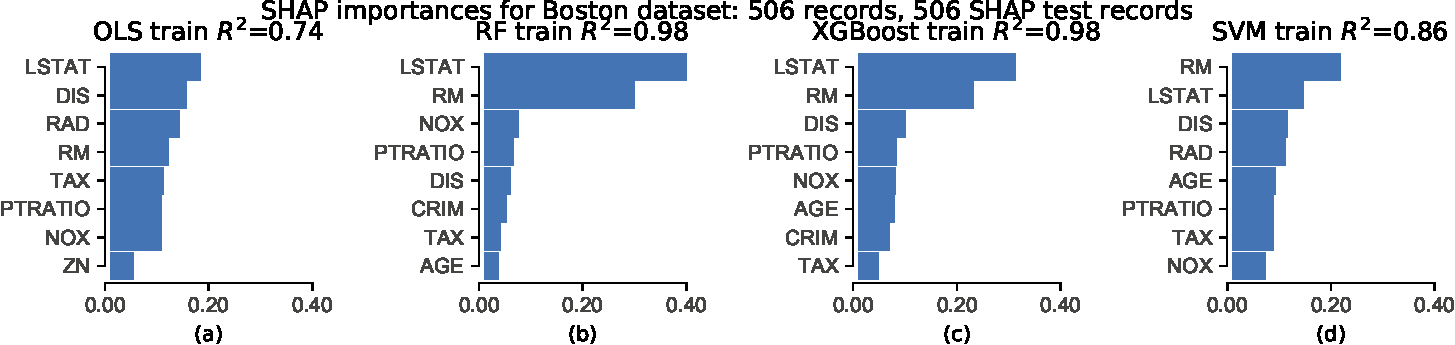
\includegraphics[scale=0.6]{images/diff-models.pdf}
\caption{Top 8 of 13 features. {\tt\footnotesize RandomForestRegressor(n\_estimators=30)}, {\tt\footnotesize XGBRegressor(max\_depth=5, eta=0.01, n\_estimators=50)}, {\tt\footnotesize SVR(gamma=0.001, C=100)} High var for RF. nshap=n test records. Rough timing for explaining 506 test records is (a) less than 1 second, (b) 10s, (c) 3s, and (d) 50s.}
\label{fig:diff-models}
\end{center}
\end{figure}

The differences clearly arise because the feature importances are distorted by the lens' of the models, but true feature importances are relationships that exist in the data, with or without a model.  For example, to gain business insights about customers, a predictive model is unnecessary and a data analysis technique that revealed importances directly from the data would be sufficient and preferable.  Besides, predictive features do not always coincide with important features; e.g., some models are unable to capture nonlinear relationships and, therefore, always find such features unimportant.  \todo{last bit redundant?}
 
In our experience, it is best to get importances using multiple techniques and to view the combined results as a clue rather than the gospel truth.  The unfortunate reality, though, is that practitioners routinely make business decisions and  perform feature selection using the results provided by machine learning libraries without questioning their validity.  For example, \cite{rfpimp} demonstrated that the widely-used {\em gini-drop} technique, specific to random forests and provided by the popular {\tt scikit-learn} Python library, gives inappropriate weight to features with many unique values, even pure noise features. (The gini-drop of a feature is the average drop in gini impurity for decision nodes splitting on that feature.) \todo{transition}

Despite many years of research attention, there is still no widely-accepted definition of feature importance. While there are multiple precisely-defined algorithms, we are unaware of a purely mathematical, data-driven, non-algorithmic definition.  Existing model-free techniques are greedy feature-selection algorithms rather than formulas to compute importances. Model-based techniques observe model behavior to estimate feature importances but, by definition, such estimates contain both feature importance and predictive strength information for a specific model.  The primary contributions of this paper are (1) a simple, intuitive, and mathematical formula for computing feature importance that is purely a function of training data and (2) an efficient implementation that yields plausible and effective results, as measured by the model prediction error for the top $k$ features (\secref{sec:experiments}). \todo{probably need to say regression versus classifier here.}

~\\
\noindent \todo{Likely a good spot for a paper walk-through}

\section{The definition of feature importance}\label{sec:def}

Practitioners loosely define feature importance as feature predictiveness, which presupposes a fitted predictive model, probably because importances are so often used for feature selection during model development.  Research  focuses on more accurately identifying the impact of features upon model predictions.  But, relying on a fitted model makes it difficult to tease apart the true feature importance from the ability of the model to exploit that feature for prediction purposes. Rather than measuring feature impact on {\em model predictions}, we propose avoiding the model completely to define feature importance as the average impact of a feature on the {\em data set response values}.

In special circumstances, we know the precise importance of each feature $x_j$. Assume we are given training data pair ($\bf X, y$) where ${\bf X} = [x^{(1)}, \ldots, x^{(n)}]$ is an $n \times p$ matrix whose $p$ columns represent observed features and ${\bf y}$ is the $n \times 1$ vector of responses.  If a data set is generated using a linear function, $y = \beta_0 + \sum_{j=1}^p \beta_j x_j$, \todo{assumes independence of $x_j$?} then coefficient $\beta_j$ corresponds exactly to the importance of $x_j$.  $\beta_j$ is the impact on $y$ for a unit change in $x_j$, holding all other features constant.

To hold features constant for any smooth generator function, we can take the partial derivatives of $y$ with respect to each feature $x_j$. For any smooth function $f:\mathbb{R}^{p} \rightarrow \mathbb{R}$ that precisely maps each $\xi$ to $y_i$, ${y_i} = f(\xi)$, \todo{should that be $y^{(i)}$ to be consistent?} the partial derivative of $y$ with respect to $x_j$ gives the change in $y$ holding all other variables constant; e.g., for linear functions, $\frac{\partial y}{\partial x_j}=\beta_j$. Integrating the partial derivative then gives the {\em partial dependence}  of $y$ on $x_j$, the isolated contribution of $x_j$ to $y$. But, rather than relying on a fitted model as originally formulated by \cite{PDP}, this definition of partial dependence relies on the partial derivative of a known function that generated the data set.

~\\
\noindent {\bf Definition 1} The model-free partial dependence of $y$ on feature $x_j$ for smooth generator function $f:\mathbb{R}^{p} \rightarrow \mathbb{R}$ evaluated at $x_j = z$ is the cumulative sum up to $z$:

\begin{equation}\label{eq:pd}
\text{\it PD}_j(z) = \int_{min(x_j)}^z \frac{\partial y}{\partial x_j} dx_j
\end{equation}

$\text{\it PD}_j(z)$ is the value contributed to $y$ by $x_j$ at $x_j = z$. The advantage of this partial dependence definition is that it is insensitive to collinear or otherwise codependent features, unlike the traditional definition that is most accurate for fitted models ``{\em dominated by low order interactions}'' per Friedman.  

To go from partial dependence to feature importance, we compare the area under each partial dependence curve. The larger the area under the curve, the larger the impact on $y$.   By the mean-value theorem of integrals, the area under $f(x)$ in interval $[a,b]$ is $\int_{a}^{b} f(x) dx = \overline{f(x)}(b-a)$.  For comparison purposes between variables, the actual area is not important and the $b-a$ term drops out, if we normalize the variables so all $x_j$ domains have the same range, such as $[0,1]$. The importance of $x_j$ is then just the average magnitude of $\text{\it PD}_j(x_j)$.

~\\
\noindent {\bf Definition 2a} The feature importance of $x_j$ is the ratio of $x_j$'s average partial dependence value to the total of all variables, when all $x_j$ variables are normalized to the same fixed range:

\begin{equation}\label{eq:Epd2a}
\Imp_j = \frac{\overline{|\text{\it PD}_j|}}{\sum_{k=1}^p \overline{|\text{\it PD}_k|}}
\end{equation}

\noindent For example, consider quadratic equation $y = x_1^2 + x_2 + 100$ as a generator of data in $[0,3]$. The partial derivatives are $\frac{\partial y}{\partial x_1} = 2 x_1$ and $\frac{\partial y}{\partial x_2} = 1$, giving $\text{\it PD}_1 = x_1^2$ and $\text{\it PD}_2 = x_2$. The areas under the partial dependence curves in $[0,3]$ are $\Imp_1 = \frac{x_1^3}{3} \big |_0^3 = 9$ and $\Imp_2 = \frac{x_2^2}{2} \big |_0^3 = 4.5$.   Therefore, $x_1$ is twice as important as $x_2$ for data generated in that interval with importances $\Imp_1 = 0.\overline{66}$ and $\Imp_2 = 0.\overline{33}$. \figref{fig:quad-area} shows...


\begin{figure}[htbp]
\begin{center}
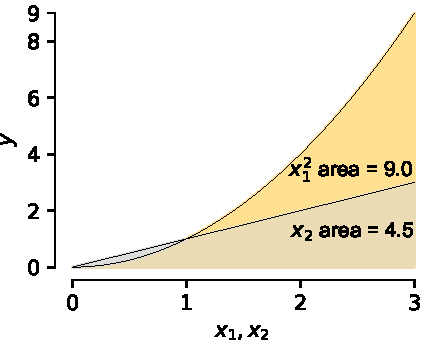
\includegraphics[scale=0.6]{images/quadratic-auc.pdf}
\captionof{figure}{\small AUC for partial dependence curves from $y = x_1^2 + x_2 + 100$ in $[0,3]$}
\label{fig:quad-area}
\end{center}
\end{figure}

The obvious disadvantage of this feature importance definition is that function $f$, from which $\text{\it PD}_j$ is derived, is unknown in practice, so symbolically computing the partial derivatives is not possible. But, if we could compute accurate partial dependence curves by some other method, then this definition would still represent a viable means to obtain true feature importances. 

As originally defined, partial dependence curves are derived from fitted models and are biased in the presence of codependent variables.  To overcome this bias and to avoid the need for predictions from a fitted model, we recently introduced a technique called \spd{} (\cite{stratpd}) to approximate partial dependence curves using a data stratification approach. \spd{} stratifies a data set into groups of observations that are similar, except in the variable of interest, $x_j$, through the use of a single decision tree. Any fluctuation of the response variable within a group (decision tree leaf) is likely due to $x_j$. The $\beta_1$ coefficient of a simple local linear regression fit to the $(x_j, y)$ values within a group provides an estimate of $\frac{\partial y}{\partial x_j}$ in that group's $x_j$ range. Averaging the partial derivative estimates across all such groups yields the overall $\frac{\partial y}{\partial x_j}$ partial derivative approximation. The cumulative sum of the partial derivative yields the partial dependence curve. (Note that \spd{} never uses predictions from any model---the decision tree merely stratifies feature space and the piecewise linear regression models provide slope estimates.)

\begin{minipage}[t]{0.35\textwidth}
\centering
\vspace{1em}
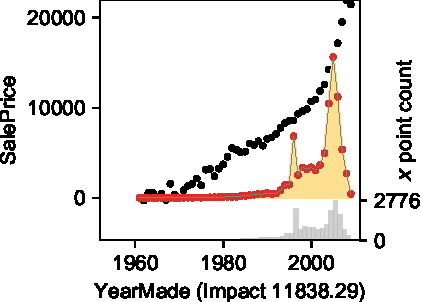
\includegraphics[scale=0.7]{images/bulldozer-impact-YearMade.pdf}\captionof{figure}{AUC for bulldozer features weighted by evidence, 20, 000 records of 401,125}
\label{fig:bulldozer-impact}
\end{minipage}

The definition of $\Imp_j$ in \eqnref{eq:Epd2a} assumes that data is evenly distributed across all $x_j$ domains, which is not the case in practice for $(\bf X, y)$ data sets.  The impact of each $\text{\it PD}_j$ curve value must be weighted by the number of samples at $x_j=z$.  For example, \figref{fig:bulldozer-impact} shows the partial dependence curve (black dots) for feature {\tt\small age} from the bulldozer auction data set \cite{bulldozer}. The gray histogram under the curve indicates the number of samples at each $x_j$ value. The red dots represent the $\text{\it PD}_j$ weighted according to the histogram height and the orange region represents the impact {\tt\small YearMade} has on target {\tt\small SalePrice}. While the {\tt\small YearMade} partial dependence curve is plausible before year 1990 (older bulldozers are worth less), there are so few data points that the collection of very old bulldozers should have little overall effect on the overall average sale price.  This leads to a definition based upon expected value rather than simple averages across $x_j$ domains.

~\\
\noindent {\bf Definition 2b} The feature importance of $x_j$ is the ratio of $x_j$'s expected partial dependence value to the total of all expected values, when all $x_j$ variables are normalized to the same fixed range:


\begin{equation}\label{eq:Epd2b}
\Imp_j = \frac{\Ex[|\text{\it PD}_j|]}{\sum_{k=1}^p \Ex[|\text{\it PD}_k|]}
\end{equation}

\noindent where:

\begin{equation}\label{eq:Epd2c}
\Ex[|\text{\it PD}_j|] = \frac{1}{n} \sum_{i=1}^{n} |\text{\it PD}_j(x_j^{(i)})|
\end{equation}

\todo{
\begin{itemize}
\item Do we need to explain why that is a weighted sum? i.e., repeated $x_j^{(i)}$ values and in repeated partial dependence values.
\item in our case $n$ differs for each $x_j$ due to implementation details of \spd{} but in the general case can't we therefore remove that common factor and just say that the weighted sum relative to other variables' weighted sum is the importance?
\item do we need to point out that $\sum_{k=1}^p \Ex[|\text{\it PD}_k|]$ is not the expected value of avg $|y|$? I.e., why are we not dividing by avg $|y|$?
\end{itemize}
}

Intuitively, the feature importance of $x_j$ is how much, on average, the values of $x_j$ are expected to push $y$ away from zero. We deliberately chose this  definition instead of measuring how much $x_j$ pushes $y$ away from the average response, $\overline{y}$. The impact of $x_1$ on $y$ is $x_1^2$, not $\overline{y} - x_1^2$; e.g., at $x_j=0$, the impact on $y$ should be 0, not $\overline{y}-0 = \overline{y}$.  \figref{fig:combined-area} illustrates how the area under the $x_1^2$ and $x_2$ partial dependence curves from $y = x_1^2+x_2+100$ differ from the area straddling the means. The true area under the curve ratio of $x_1$-to-$x_2$ is 2-to-1 (9/4.5), whereas the ratio of the area straddling the mean has roughly a 3-to-1 ratio (6.95/2.26). \todo{is this clear enough?}
 
\section{Existing methods}

Feature importance methods for labeled data sets (with $\bf X$ and $\bf y$) are broadly categorized into data analysis and model analysis techniques, sometimes called {\em filter} and {\em wrapper} methods. Data analysis techniques analyze the data directly to identify important features, whereas model analysis techniques rely on predictions from fitted models.  The intended application of the feature importances (business insight or feature selection) often dictates the approach.  The data analysis techniques further split into techniques for regression and techniques for classification, with most of the research going into classification.

The simplest technique to identify important regression features is to rank them by their Spearman's rank correlation coefficient \cite{spearmans}; the feature with the largest coefficient is taken to be the most important. This method works well for independent features, but suffers in the presence of codependent features.   Groups of features with similar relationships to the response variable receive the same or similar ranks, even though just one should be considered important.

Another possibility is to use principle component analysis (PCA), which operates on just the $\bf X$ explanatory matrix. PCA transforms data into a new space characterized by eigenvectors and identifies features that explain the most variance in the new space. If the first principal component covers a large percentage of the variance, the ``loads'' associated with that component can indicate importance of features in the original $\bf X$ space. PCA is limited to linear relationships, however, and ``most variation'' is not always the same thing as ``most important.''

For classification data sets, the Relief algorithm (\cite{relief}) tries to identify features that distinguish between classes through repeated sampling of the data. For a sampled observation $\xi$, the algorithm finds the nearest observation with the same class (hit) and the nearest observation with the other class (miss). The score of each attribute, $x_j$, is then updated according to the distance from the selected $\xi$ to the hit and miss observations'  $x_j$ values. ReliefF \cite{ReliefF} extended Relief to work on multiclass problems and RReliefF \cite{RReliefF} adapted the technique to regression problems (by ``...introduc[ing] a kind of probability that the predicted values of two instances are different'').

In an effort to deal with codependencies, data analysis techniques rank features not just by {\em relevance} (correlation with the response variable) but also by low {\em redundancy}, the amount of information shared between codependent features, which is the idea behind minimal-redundancy-maximal-relevance (mRMR) by \cite{mRMR}. mRMR selects features in order according to the following score.

\[
J_{mRMR}(x_k) = I(x_k, y) - \frac{1}{|S|} \sum_{x_k \in S} I(x_k, x_j)
\]

\noindent where $I(x_k, x_j)$ is some measure of mutual information between $x_k$ and $x_j$, $S$ is the growing set of selected features, and $x_k$ is the candidate feature. mRMR only considers pairwise codependencies between features and is limited to classification as originally defined. See \cite{ubermRMR} for a recent application of mRMR at Uber Technologies.  For more on model-free feature importances, see the survey by \cite{survey}.

Turning to model-based techniques, feature importances are typically variations on a theme: tweak the model and measure the effect on model prediction accuracy or expected model output. The simplest approach is {\em drop-column importance}, which defines $x_j$ importance as the difference in model accuracy between the full model and the model with $x_j$ removed. The model must be retrained $p$ times and highly similar features yield low or zero importances because codependent features cover for the dropped column in the model.

To avoid retraining the model, $x_j$ can be permuted instead of dropped for {\em permutation importance} (\cite{RF}). This approach is faster but can introduce nonsensical observations by permuting invalid values into records; e.g., shifting a true {\tt\small pregnant} value into a male's record. Codependent features tend to share importance, at least when applied to random forest models.

Rather than removing or permuting entire columns of data, LIME \cite{lime} and SHAP \cite{shap} focus on model behavior at the observation level. For a prediction of interest, LIME trains an interpretable linear model, on a small neighborhood of data around that prediction to explain the relationship between variables and the response locally. SHAP, however, was shown to subsume the LIME technique in \cite{shap}.

SHAP has its roots in {\em Shapley regression values} \cite{shapley-regression} where (linear) models are trained on all possible subsets of features.  Each possible model pair differs in a single feature $x_j$ and contributes the difference in model pair output towards the Shapley value for $x_j$. The complete Shapley value is the average model-pair difference weighted by the number of possible pairs differing in just $x_j$.  For completely independent features, drop-column importance is sufficient because the contribution of $x_j$ can be computed without considering how combinations of features affect model output.  In practice, features are rarely independent and the marginal effect of adding a new feature on model output depends on the order in which features are added.  

To avoid training a combinatorial explosion of models with the various feature subsets, SHAP reuses the same model by running simplified feature vectors into the model. Simplified vectors replace ``missing'' $x_j$ features with the expected value of $x_j$, to simulate models trained on feature subsets. To further reduce computation costs, SHAP computes values on a subsample from the data set. SHAP has model-type-dependent optimizations for linear regression, deep learning, and decision-tree based models. As with permutation methods, replacing feature values with their expectations introduces the possibility of creating nonsensical feature vectors; e.g., replacing a bulldozer {\tt\small age} feature with the average risks conjuring up a type of bulldozer that did not exist at that time. This causes errors in contribution of var to y. 

\begin{figure}[htbp]
\begin{center}
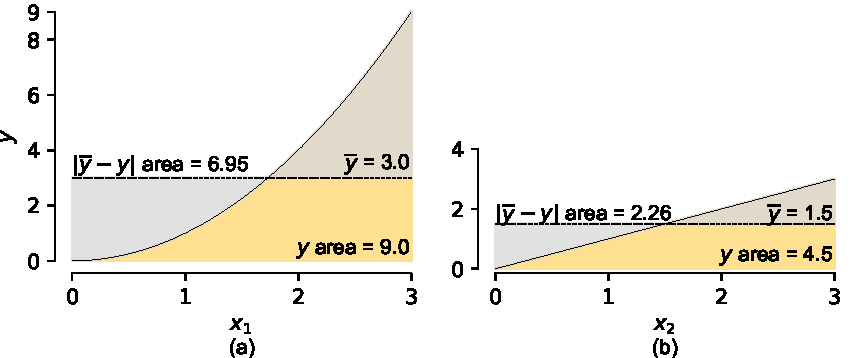
\includegraphics[scale=0.65]{images/from-mean-auc.pdf}
\captionof{figure}{AUC for partial dependence curves from $y = x_1^2 + x_2 + 100$ in $[0,3]$ Shows why must compute from 0 not deviation from mean}
\label{fig:combined-area}
\end{center}
\end{figure}

 disadvantages are the subsets  size too small to be representative and costs go up dramatically. this is not a problem for linear models; SVM took 13min. RF goes up. boosting faster as it has shallower trees.
 
Equation (7) from \cite{stratpd} 

\begin{equation}\label{eq:weight}
y_{weight}  = 120 + 10(x_{height} - min(x_{height})) + 30x_{pregnant} - 1.5x_{education}
\end{equation}

where the relationship between height and weight and women gaining 70 pounds to make the bias more prominent. \figref{fig:shap-weight} show ...  \spd{} gives a flat line with slope with roughly 10 (see \cite{stratpd} for more).

\begin{figure}[htbp]
\begin{center}
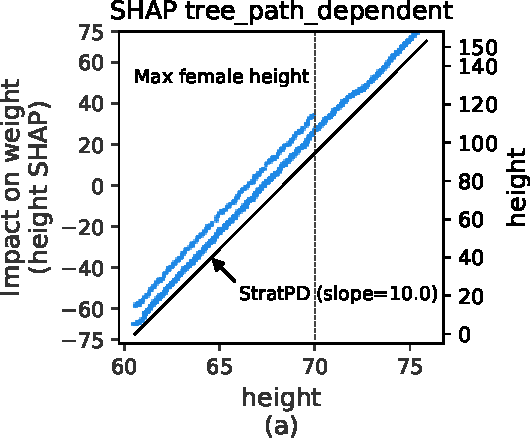
\includegraphics[scale=0.7]{images/weight-shap-tree_path_dependent.pdf}~~
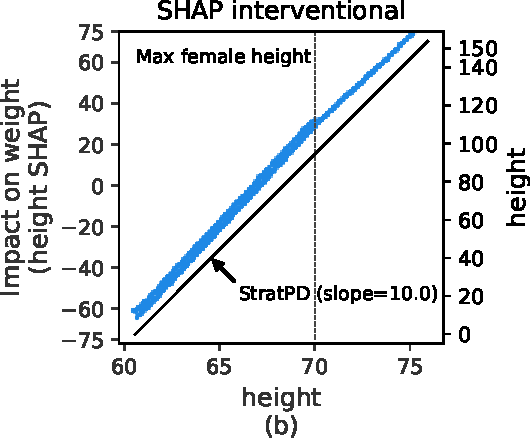
\includegraphics[scale=0.7]{images/weight-shap-interventional.pdf}
\caption{Plots of height versus body weight using 2000 observations from Equation \eqref{eq:weight} as drawn by SHAP library}
\label{fig:shap-weight}
\end{center}
\end{figure}

\begin{figure}[htbp]
\begin{center}
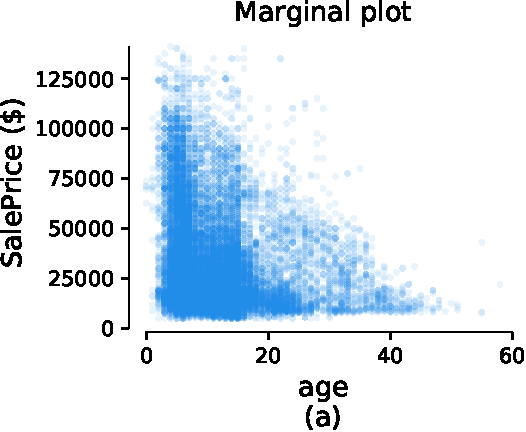
\includegraphics[scale=0.6]{images/bulldozer-age-marginal.pdf}~~
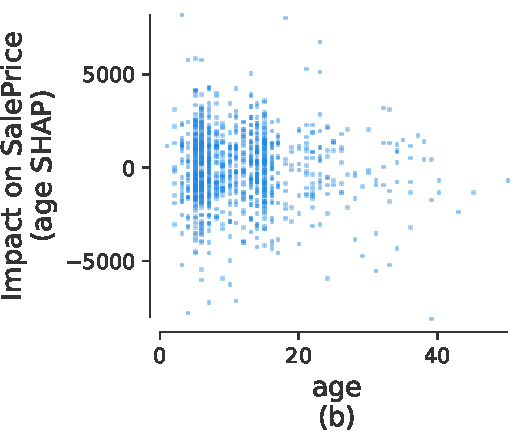
\includegraphics[scale=0.6]{images/bulldozer-age-shap.pdf}~~
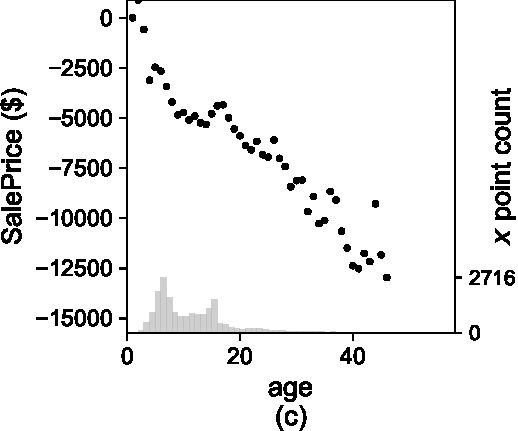
\includegraphics[scale=0.6]{images/bulldozer-age-stratpd.pdf}
\caption{Bulldozer age vs SalePrice, as drawn by SHAP library and StratPD}
\label{fig:shap-stratpd-age}
\end{center}
\end{figure}

SHAP has model type optimizations so it is for performance; not unlike gini drop it is sensitive to vagaries of the underlying model.  high variance models such as the decision trees inside random forests can lead to high variance of SHAP values.

most approaches are model-independent
 
LIME has a linear model that approximates the output in a neighborhood of x for each x. this might be the Segway to gini drop and model type dependent SHAP.

SHAP replaces missing values with mean, which can create nonsensical and what do they do with categoricals?

\todo{ do we need to mention LASSO?}

Here is where we show that SHAP gets $y = x_1^2 + x_2 + 100$ wrong.



\section{Experimental results}\label{sec:experiments}

\todo{an experiment where we show insensitive to noise column and any other codependent ones that are thrown in but don't affect y}

\todo{maybe show the linear 1 1 1 codependence example}

\todo{what about outlier example}

\todo{stability is valuable. users would not trust results that changed significantly for small data set changes. show our error bars from bootstrapping and say we can do p-values.}

\todo{bulldozer: YearMade ignores too much with stratpd, use catstrat}

Even with domain expertise, humans are unreliable estimates of feature importance. Otherwise, we would need feature important mechanisms. Comparing the quality of feature importance methods is then a challenge. The simplest approach is to compare methods on synthetic data for which the answer is clear, such as the quadratic in \ref{eq:quad}.

For real data sets, we can train a predictive model on the most important $k$ features and compare prediction error. The importance method that accurately identifies the most impactful features without getting confused by codependent features, should yield lower production errors for a given $k$.   This mirrors how one would use it for model feature selection.
 
The best feature importance method ranks features by their independent contributions to $y$, without getting confused by codependent features. The most important single feature as reported by two importance methods can be used to train a model and measure a prediction metric.
 
{\bf Definition 3} The {\em top-k} fitness measure trains a suitable model on the  most important $k$ features as reported by two or more importance methods then compares prediction metrics. Actually p246 \cite{liu-fs} has an example of this.

even if recommendations are identified by their isolated contribution, the model is still taking the combination into consideration when fitting and hence the marginal errors are not necessarily reduced specifically because of the added feature at number $k$.

Get a baseline \figref{fig:baseline}.

\begin{figure}
\centering
\begin{subfigure}{.24\textwidth}
    \centering
\includegraphics[scale=0.51]{images/boston-topk-spearman.pdf}
\subcaption{\footnotesize foo}
\end{subfigure}%
\hfill
\begin{subfigure}{.24\textwidth}
    \centering
\includegraphics[scale=0.53]{images/flights-topk-spearman.pdf}
\subcaption{\footnotesize foo}
\end{subfigure}
\hfill
\begin{subfigure}{.24\textwidth}
    \centering
\includegraphics[scale=0.53]{images/bulldozer-topk-spearman.pdf}
\subcaption{\footnotesize foo}
\end{subfigure}
\hfill
\begin{subfigure}{.24\textwidth}
    \centering
\includegraphics[scale=0.44]{images/rent-topk-spearman.pdf}
\subcaption{\footnotesize foo}
\end{subfigure}
\caption{Whew}
\label{fig:baseline}
\end{figure}

Model-based methods have all the advantages in these experiments.

In \figref{fig:features}, we

Then see \figref{fig:topk}

\begin{figure}
\centering
\begin{subfigure}{.24\textwidth}
    \centering
\includegraphics[scale=0.48]{images/boston-topk.pdf}
\subcaption{\footnotesize foo}
\end{subfigure}%
\hfill
\begin{subfigure}{.23\textwidth}
    \centering
\includegraphics[scale=0.48]{images/flights-topk.pdf}
\subcaption{\footnotesize sometimes we get age as first feature which is ok but not the amazing ModelID, clearly best.}
\end{subfigure}
\hfill
\begin{subfigure}{.25\textwidth}
    \centering
\includegraphics[scale=0.5]{images/bulldozer-topk.pdf}
\subcaption{\footnotesize foo}
\end{subfigure}%
\hfill
\begin{subfigure}{.2\textwidth}
    \centering
\includegraphics[scale=0.5]{images/rent-topk.pdf}
\subcaption{\footnotesize foo}
\end{subfigure}
\caption[short]{A caption}
\label{fig:topk}
\end{figure}

\begin{figure}
\centering
\begin{subfigure}{1\textwidth}
    \centering
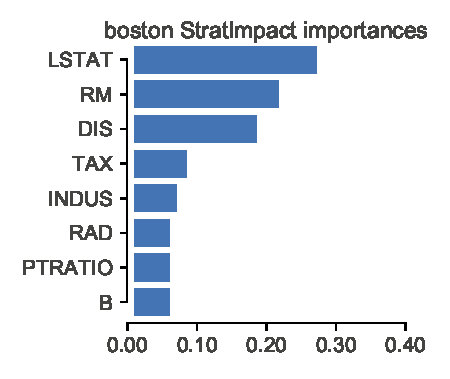
\includegraphics[scale=0.6]{images/boston-features.pdf}
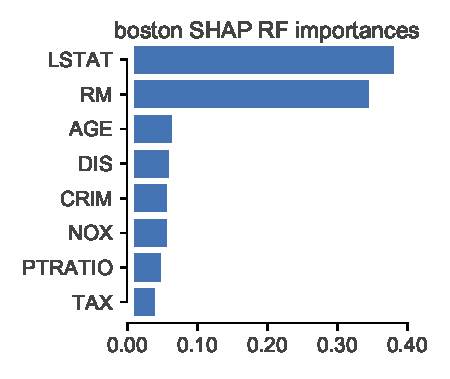
\includegraphics[scale=0.6]{images/boston-features-shap-rf.pdf}
\vspace{-2mm}\subcaption{\footnotesize Note LSTAT/RM order is diff than in original figure as their is high variance}\vspace{3mm}
\end{subfigure}%
\hfill
\begin{subfigure}{1\textwidth}
    \centering
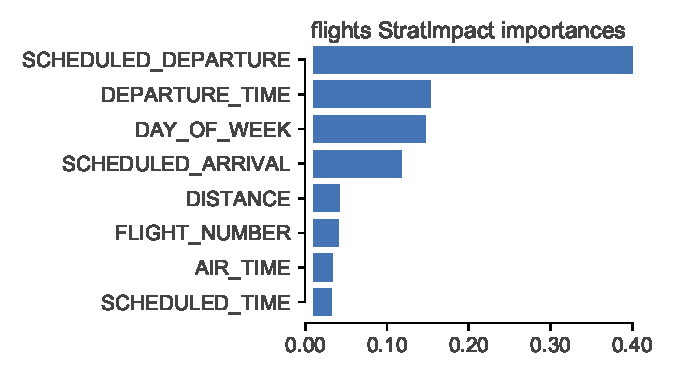
\includegraphics[scale=0.6]{images/flights-features.pdf}
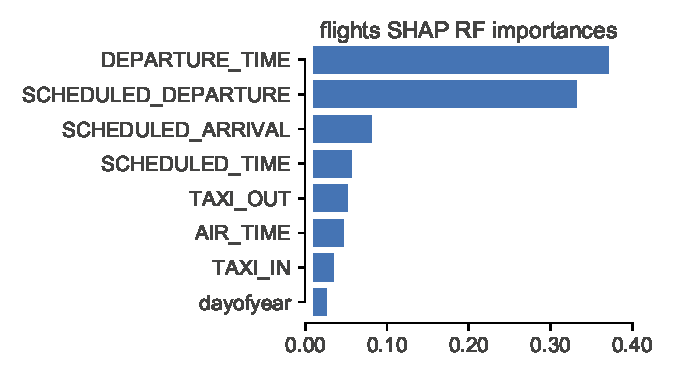
\includegraphics[scale=0.6]{images/flights-features-shap-rf.pdf}
\vspace{-2mm}\subcaption{\footnotesize 5.8M records}\vspace{3mm}
\end{subfigure}
\hfill
\begin{subfigure}{1\textwidth}
    \centering
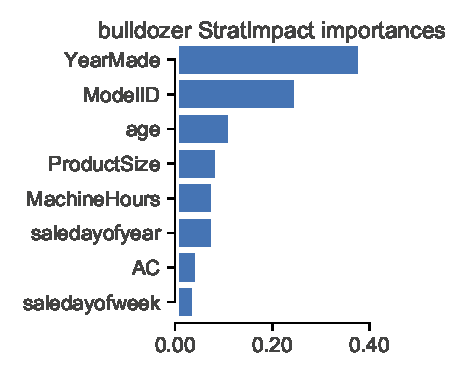
\includegraphics[scale=0.6]{images/bulldozer-features.pdf}
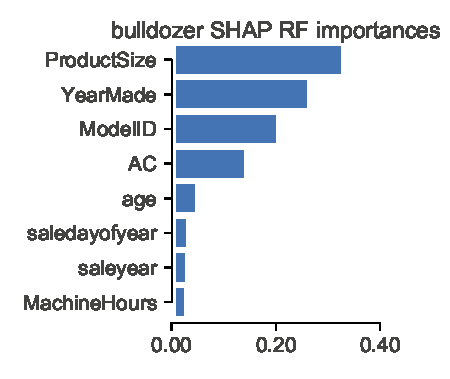
\includegraphics[scale=0.6]{images/bulldozer-features-shap-rf.pdf}
\vspace{-2mm}\subcaption{\footnotesize foo}\vspace{3mm}
\end{subfigure}%
\hfill
\begin{subfigure}{1\textwidth}
    \centering
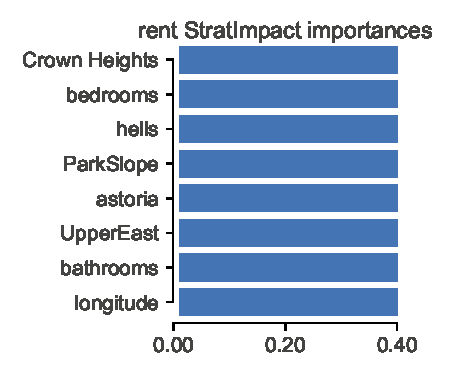
\includegraphics[scale=0.6]{images/rent-features.pdf}
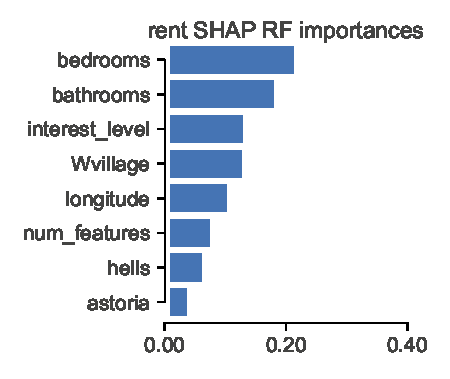
\includegraphics[scale=0.6]{images/rent-features-shap-rf.pdf}
\vspace{-2mm}\subcaption{\footnotesize foo}\vspace{3mm}
\end{subfigure}
\caption[short]{blorttttt}
\label{fig:features}
\end{figure}

Consider the recommendations from OLS SHAP used in a random forest. In general, they are not good recommendations. This demonstrates that the rank of features is highly dependent upon the model used to get those recommendations. In some cases, plain OLS recommendations fitted to RF beats the recommendations from OLS SHAP fitted to the RF.

Do an experiment that compares PCA and Spearman's R against StratImpact.

performance. with lots of outliers, choosing a small subset for shap is a bad idea so this is a real problem. linear and boosted trees are efficient but RF are not and I wouldn't consider anything using the general explainer.

There are issues surrounding how many explanatory samples you can use. 300 even run a couple of times is not enough to sample 5.8M records.

\todo{We need min samples per x to avoid left edge issues as they skew entire pdp, which severely skews mass AUC.}

\todo{explain cat mechanism and how there is no left/right edge so no evidence used to weight AUC.}
 
\section{foo}

 what is the definition: loosely as which are most predictive

The variance of the importances derived from the random forest is high, SHAP has specialized ``explainers'' for linear and tree-based models for performance reasons, but relies on the general method to explain support vector machines. , but the results are subject to the variance of the internal model parameters.  Ideally, feature importances would not change from run to run on the same data set using the same technique.

\section{Discussion and future work}

We deal with all possible combinations for codependency's because of the nature of the partial dependence mechanism.

features important in one model are not exportable to another which also means that they're less likely to be useful for business insight.
 
For business insight purposes, practitioners often favor direct data analysis, but to perform machine learning model feature selection, practitioners strongly favor model-based techniques. The idea being that business insight should flow directly from the data without peering through a (possibly unneeded) predictive model.  Similarly, it stands to reason that computing feature importances using the intended predictive model would provide the most useful ranking.

Our experience is that model analysis techniques dominate in practice, even for business insight purposes. Part of this is due to the prevalence of machine learning model usage but is also because we conflate predictive with important.  Predictiveness is sometimes a function of the model choice, however, rather than the inherent importance of the feature. For example, there could be a complex but one-to-one relationship between a variable and the response variable. A model unable to capture that relationship would show it as unpredictive, which is easy to confuse with unimportant.  On the other hand, important or not, tuning a model using what it considers predictive is useful in practice. Consequently, it might make sense to continue the bifurcation between data analysis for business insight and model analysis for model feature selection.

research should now focus on getting more accurate partial dependence approximations.

must define for classification

\bibliographystyle{apalike}

\bibliography{pdimp}
\end{document}